\documentclass[10pt,a4paper]{article}
\usepackage[utf8]{inputenc}
\usepackage[T1]{fontenc}
\usepackage{amsmath}
\usepackage{amssymb}
\usepackage{graphicx}

\newtheorem{theorem}{Theorem}
\newtheorem{definition}{Definition}
\usepackage{algorithm}
\usepackage{algpseudocode}
\usepackage{listings, lstautogobble}
\lstset{
	language=Matlab, autogobble=true
}
\title{Numerik MA0008: Zusammenfassung}
\author{Jonas Treplin}
\begin{document}
	\maketitle
	\section{Grundlagen}
	\begin{theorem}[Satz von Gerschgorin]
		Sei $(a_{ij})=A \in \mathbb{R}^{n\times n}$ dann sind die Eigenwerte von $A$ enthalten in $\bigcup_{i=1}^{n}S_i \subset \mathbb{C}$, dabei sind die $S_i := K(a_{ii}, \sum_{j=1, i\neq j}^{n})$. Wobei mindestens ein Eigenwert jeder Zusammenhangskomponente zugeordnet ist.
	\end{theorem}
	\section{Matrixfaktorisierung}
	\subsection{Lösen einfacher Matrizen}
	\begin{theorem}
		Die Permutationsmatrizen, die unitären Matrizen, die invertierbaren Matrizen und die unteren/oberen Dreiecksmatrizen bilden jeweils unter Matrixmultiplikation eine Gruppe. Insbesondere sind ihre Inverse von der selben Klasse von Matrizen. 
	\end{theorem}
	Gleichungssysteme für die unitären Matrizen (und damit auch Permutationsmatrizen) lassen sich einfach durch adjungieren lösen. Für untere und obere Dreiecksmatrizen existieren Vorwärts- und Rückwärtssubsitution.  Diese sind aus dem Endschritt des Lösens von Gleichungssystemen mit dem Gauß-Algorithmus bekannt.
	\begin{algorithm}
		\caption{Vorwärtssubsitution (Lösen einer unteren Dreiecksmatrix)}
		\begin{algorithmic}
			\Require $(l_{ij}) = L \in \mathbb{R}^{n\times n}$ Untere Dreiecksmatrix, $b \in \mathbb{R}^n$.
			\For{$i\in 1:n$}
				\State $x_i \leftarrow \frac{1}{l_{ii}}(b_i - \sum_{j=1}^{i-1}l_{ij}*x_j)$
			\EndFor
		\end{algorithmic}
	\end{algorithm}
	\begin{algorithm}
		\caption{Rückwärtsssubsitution (Lösen einer oberen Dreiecksmatrix)}
		\begin{algorithmic}
			\Require $(u_{ij}) = U \in \mathbb{R}^{n\times n}$ Obere Dreiecksmatrix, $b \in \mathbb{R}^n$.
			\For{$i\in n:1$}
			\State $x_i \leftarrow \frac{1}{u_{ii}}(b_i - \sum_{j=i+1}^{n}u_{ij}*x_j)$
			\EndFor
		\end{algorithmic}
	\end{algorithm}
	\subsection{LU-Zerlegung}
	Glücklicherweise kann jede invertierbare Matrix (fast eindeutig) in solche Matrizen zerlegt werden. Dies geschieht Wahlweise durch eine LU-Zerlegung oder eine QR-Zerlegung.
	\begin{algorithm}
		\caption{LU-Zerlegung ohne Pivots}
		\begin{algorithmic}
			\Require $(a_{ij}) = A \in GL(n)$
			\For{$i\in 1:n$}
				\State $l_{ii} \leftarrow 1$
				\For{$j \in i+1:n$}
					\State $l_{ji} \leftarrow -\frac{a_{ji}}{a_{ii}}$
					\For{$k\in i:n$}
						\State $a_{jk} \leftarrow a_{jk} - a_{ji}a_{ji}$
					\EndFor
				\EndFor
			\EndFor
			\State $U = triu(A)$
		\end{algorithmic}
	\end{algorithm}
	Mit Pivots erreicht man, dass jede invertierbare Matrix $A \in GL(n)$ zerlegt werden kann, sodass $PA = LU$. Dazu wählt man in jedem Schritt $i$ die Zeile $j = \arg \max_{j\geq i} |a^i_{ji}|$ und vertauscht diese mit der $i$-ten Zeile. 
	\begin{algorithm}[H]
		\caption{LU-Zerlegung mit Pivots}
		\begin{algorithmic}
			\Require $(a_{ij}) = A \in GL(n)$ 
			\State $P = Id$
			\For{$i\in 1:n$}
				\State $p \leftarrow\arg\max_{i\leq k\leq n} |a_{ki}|$
				\State $P, A, L \leftarrow P^{(p, i)} P, P^{(p, i)}A, P^{(p, i)}L$
				\State $l_{ii} \leftarrow 1$
				\For{$j \in i+1:n$}
					\State $l_{ji} \leftarrow -\frac{a_{ji}}{a_{ii}}$
					\For{$k\in i:n$}
					 	\State $a_{jk} \leftarrow a_{jk} - a_{ji}a_{ji}$
					\EndFor
				\EndFor
			\EndFor
			\State $U = triu(A)$
		\end{algorithmic}
	\end{algorithm}
	\begin{theorem}[LU-ZErlegung mit Pivots]
		Sei $A \in GL(n)$. Dann existieren eine eindeutige Permutationsmatrix $P$, sowie untere (obere) Dreiecksmatrix $L$ ($U$, sodass $PA =LU$. Dabei ist $L$ normiert also $l_{ii}= 1$.
	\end{theorem}
	\begin{theorem}
		Für s.p.d. Matrizen sowie spalten-/zeilendiagonaldominante Matrizen ist keine Pivotsuche notwendig.
	\end{theorem}
	\begin{theorem}[Cholesky-Zerlegung]
		Sei $A$ symmetrisch positiv definit dann lässt sich eine nicht normierte untere Dreiecksmatrix $\tilde{L}$ finden, sodass $A = \tilde{L}\tilde{L}^T$.
	\end{theorem}
	\begin{algorithm}
		\caption{Berechnung der Cholesky Zerlegung}
		\begin{algorithmic}
			\Require $A$ s.p.d.
			\State $L, U \leftarrow \text{LU\_Zerlegung(A)}$
			\State $D = (u_{ii})$ Diagonalmatrix.
			\State $\tilde{L} = \sqrt{D}L$.
		\end{algorithmic}
	\end{algorithm}
	\subsection{QR-Zerlegung}
	Eine weitere Möglichkeit ist die der $QR$ Zerlegung. 
	\begin{definition}[Givensrotation]
		Für ein $a \in \mathbb{R}^2$ sei $Q=\begin{bmatrix}
			c & s \\
			-s & c
		\end{bmatrix}$. Wobei $c=\frac{1}{\sqrt{1+\tau^2}}$ und $s=c\tau$ mit $\tau = \frac{v_2}{v_1}$ wenn $|v_1| \geq |v_2|$ und  $s=\frac{1}{\sqrt{1+\tau^2}}$ und $c=s\tau$ mit $\tau = \frac{v_1}{v_2}$ wenn $|v_1| < |v_2|$.
	\end{definition}
	Diese Fallunterscheidung ist so gewählt, dass $||Q||\leq 1$, damit sich Rundungsfehler nicht akkumulieren.
	\begin{theorem}[Givens-Rotation]
		Es gilt $Qa = \xi e_1$.
	\end{theorem}
	\begin{algorithm}[H]
		\caption{QR-Zerlegung mit Givens-Rotationen}
		\begin{algorithmic}
			\Require $A \in \mathbb{R}^{n\times m}$
			\State $Q \leftarrow I_n$
			\For{$i \in [n]$}
				\For{$j \in (n, ..., i+1)$}
					\State $G : = \begin{bmatrix}
					1 &  &  &  &  &  \\
					& \ddots &  &  &  &  \\
					&  & c & s &  &  \\
					&  & -s & c &  &  \\
					&  &  &  & \ddots &  \\
					&  &  &  &  & 1
				\end{bmatrix} \leftarrow Givens(\begin{bmatrix}
						A_{j-1,i} \\
						A_{j-1,i}
					\end{bmatrix})$
					\State $Q \leftarrow GQ$
					\State $A \leftarrow GA$
				\EndFor
			\EndFor
			\State $Q \leftarrow Q*$
		\end{algorithmic}
	\end{algorithm}
	\begin{definition}[Householder Spiegelung]
		Die Householder Spiegelung für einen Vektor $a \in \mathbb{R}^n$ ist:
		$$Q := Id -\frac{2}{v^Tv}vv^T$$
		Wobei $v :=a+\text{sign}(a_1)||a||e_1$
		Sie erfüllt ebenfalls $Qa = \alpha e_1$
	\end{definition}
	\begin{algorithm}
		\caption{QR-Zerlegung mit Householder Rotationen}
		\begin{algorithmic}
			\Require \Require $A \in \mathbb{R}^{n\times m}$
			\State $Q \leftarrow I_n$
			\For{$i \in [n]$}
			
			\State $H \leftarrow \begin{bmatrix}
				1 & & &    \\
				& \ddots & & \\
				& & 1 & \\
				& & & \text{Householder}((a_i, ..., a_n))
			\end{bmatrix}$
			\State $Q \leftarrow HQ$
			\State $A \leftarrow HA$
			
			\EndFor
			\State $Q \leftarrow Q*$
		\end{algorithmic}
	\end{algorithm}
	Die QR-Zerlegung ist der LU-Zerlegung hinsichtlich numerischer Stabilität überlegen, besonders bei Betrachtung der Wilkinson-Matrix:
	\begin{definition}[Wilkinson-Matrix]
		Die Wilinson-Matrix ist definiert als:
		$$W_n := \begin{bmatrix}
			1 & 0 & ... & 0 & 1\\
			-1 & \ddots & ... & \vdots & \vdots\\
			\vdots& & & \ddots & \vdots\\
			-1 & ... & ... & \dots&1
		\end{bmatrix}$$
		Ein besonders instabiler Lösungsvektor ist $b_n = \begin{bmatrix}
			0\\
			\frac{1}{n}\\
			\vdots\\
			\frac{n-2}{n}\\
			1
		\end{bmatrix}$
	\end{definition}
	\begin{figure}
		\centering
		\includegraphics{"FehlerWilkinson.png"}
		\caption{Fehler beim Lösen von $W_nx =b_n$}
	\end{figure}
	\section{Fehlerrechnung}
	\begin{definition}[Fehlermaße]
		Wir definieren für eine Tupel $T= (A_1, A_2, ..., A_n)$ mit Störung $\tilde{T}=(A_+E_1, ..., A_n+E_n)$:
		\begin{itemize}
			\item das absolute Fehlermaß:
			$$[[E]]_{abs} := \max||E_i||$$
			\item das relative Fehlermaß:
			$$[[E]]_{rel}:= \max\frac{||E_i||}{||A_i||}$$
		\end{itemize}
	\end{definition}
	\begin{definition}[Maschinenepsilon]
		Das \textbf{Maschinen-$\epsilon$} is der relative Fehler, der bei Addition und Multiplikation von SKalaren auftritt. Er liegt für IEEE double-precision bei ca. $10^{-16}$
	\end{definition}
	\begin{definition}[Kondition]
		Die Kondition einer Abbildung $f$ im Punkt $x$ ist definiert als:
		$$\kappa(f, x) = \limsup_{y\to x}\frac{[[f(y)-f(x)]]}{||y-x||}$$
		Man unterscheidet zwischen:
		\begin{itemize}
			\item \textbf{gut konditionierten} Problemen: $\kappa(f,x) ~ O(1)$
			\item \textbf{schlecht konditionierten} Problemen: $\kappa(f, x) >> 1$
			\item \textbf{schlecht gestellten} Problemen: $\kappa(f, x) = \infty$
		\end{itemize}
	\end{definition}
	\begin{theorem}
		Die Kondition einer linearen Gleichung $Ax= b$ hängt nur von $A$ ab und ist:
		$$\kappa(A) = \Vert A\Vert\Vert A^{-1}\Vert$$
	\end{theorem}
	\begin{theorem}[Kondition einer $C^1$-Funktion]
		Sei $f\in C^1(D), D\subset \mathbb{R}^n$ mit $f(x)\neq 0$, dann gilt für die realtive Kondition:
		$$\kappa_{rel}(f,x) = \frac{\sum_{i=1}^n|\partial_if(x)||x_i|}{|f(x)|}$$
	\end{theorem}
	\begin{definition}[Vorwärts- und Rückwärtsfehler]
		Sei $\hat{f}$ eine numerische Näherung der Funktion $f$, dann ist an $x$:
		\begin{enumerate}
			\item Der \textbf{Vorwärtsfehler}:
			$$[[f(x)-\hat{f}(x)]]$$
			\item Der \textbf{Rückwärtsfehler}: 
			$$\inf_{\Delta x} \{[[\Delta x]] | f(x+\Delta x) = \hat{f}(x)\}$$
		\end{enumerate}
	\end{definition}
	\begin{definition}[Stabilität]
		Ein Algorithmus $\hat{f}$ zur Näherung von $f$ heißt \textbf{stabil} an $x$ bezüglich des Fehlermaßes $[[.]]$ falls ein $\tilde{x}$ existiert mit:
		$$[[x-\tilde{x}]] = O(\epsilon_m)$$
		$$[[\hat{f}(x) - f(\tilde{x})]] = O(\epsilon_m)$$
		Dabei sei $\epsilon_m$ das Maschinenepsilon.
	\end{definition}
	\begin{definition}[Rückwärtsstabilität]
		Eine Nöherung $\hat{f}$ zu $f$ heißt \textbf{rückwärtsstabil} an an $x$ bezüglich des Fehlermaßes $[[.]]$ falls ein $\tilde{x} = x+\Delta x$ existiert mit:
		$$[[x-\tilde{x}]] = O(\epsilon_m)$$
		$$\hat{f}(x) = f(\tilde{x})$$
	\end{definition}
	\begin{theorem}[Fehler rückwärtsstabiler Algorithmen]
		Der Fehler eines Rückwärtsstabilen Algorithmus $\hat{f}$ hängt nur von der Konidion von $f$ ab:
		$$[[\hat{f}]] = [[f(\tilde{x})-f(x)]] \leq c\kappa(f, x)\epsilon_m$$
	\end{theorem}
	\begin{theorem}[Rückwärtsfehler beim Lösen linearer Gleichungssysteme]
		Sei $Ax=b$ ein zu lösendes Gleichungssystem. Definiere 
		$$w(\tilde{x}) = \inf_E\{\frac{\Vert E\Vert_2}{\Vert A\Vert_2}: (A+E)\tilde{x}=b\}$$
		als den relativen Rückwärtsfehler bezüglich der Matrix $A$. Dann gilt:
		$$w(\tilde{x})=\frac{\Vert b-A\tilde{x}\Vert_2}{\Vert A\Vert_2\Vert \tilde{x}\Vert_2}$$
	\end{theorem}
	\begin{theorem}[Stabilität der Matrixmultiplikation]
		Sei $MN =A$ und $\tilde{M}, \tilde{N}$ fehlerbehaftet mit relativen Fehler kleiner als $(\delta)$, dann ist:
		$$\Vert \tilde{M}\tilde{N} - A\Vert \leq (2\delta+ \delta^2)\Vert M\Vert\Vert N \Vert$$.
		Daraus folgt, dass die QR-Zerlegung stabil bezüglich des relativen Fehlermaßes ist:
		$$\frac{\Vert \tilde{Q}\tilde{R} - A\Vert}{\Vert A\Vert} \leq \frac{1\Vert A\Vert}{\Vert A\Vert} = 1$$
		Ähnliches gilt auch für die Cholesky-Zerlegung, jedoch nciht für die LU-Zerlegung
	\end{theorem}
	\begin{algorithm}[H]
		\caption{Nachiteration}
		\begin{algorithmic}
			\Require Gleichungssystem $Ax=b$
			\State Zerlege $LU =PA$
			\State Berechne $LU\tilde{x^{(0)}= Pb}$ durch Vorwärts-/Rückwärtsssubsitution
			\For{$i=1,..., k$}
			\State Berechne $LU\Delta x^{(i)} = P(b-Ax^{(i-1)})$
			\State $x^{(i)}\leftarrow x^{(i-1)} + \Delta x^{(i)}$
			\EndFor
		\end{algorithmic}
	\end{algorithm}
	\section{Ausgleichsrechnung}
	\begin{definition}[Lineares Ausgleichsproblem]
		Sei $A\in \mathbb{R}^{n\times n}, b\in \mathbb{R}^n$ mit $m\leq n$. Gesucht ist $x\in \mathbb{R}^m$. Sodass $$||Ax-b||_2$$ minimiert wird. Es wird im Generellen angenommen, dass $Rang(A) = m$.
	\end{definition}
	\begin{definition}[Normalengleichung]
		Gegeben ein Ausgleichsproblem $A, b$, nennt man:
		$$A^TAx=A^Tb$$
		die Normalengleichung.
	\end{definition}
	\begin{theorem}[Lösung des Linearen Ausgleichproblems mittels Normalengleichung]
		Die Lösung der Normalengleichung ist das eindeutige gesuchte Minimum des Ausgleichsproblems.
	\end{theorem}
	\begin{algorithm}
		\caption{Lösen des Ausgleichproblems mittels Normalengleichung}
		\begin{algorithmic}
			\Require Ausgleichsproblem $A\in \mathbb{R}^{n\times m}, b\in \mathbb{R}^n$
			\State $L \leftarrow$ Cholesky$(A^TA)$
			\State Löse $LL^Tx = A^Tb$ durch Vorwärts und Rückwärtsssubsitution.
		\end{algorithmic}
	\end{algorithm}
	Die Stabilität des Algorithmus hängt von der Stabilität der Matrixmultiplikation $A^TA$ ab. 
	Falls $\kappa(A^TA)$ groß ist und $||Ax-b||$ klein treten hier Stabilitätsprobleme auf. Um diesen entgegen zu wirken, kann man die Orthogonalisierungsmethode verwenden.
	\begin{algorithm}
		\caption{Lösen des Ausgleichproblems mittels QR-Methode}
		\begin{algorithmic}
			\Require Ausgleichsproblem $A\in \mathbb{R}^{n\times m}, b\in \mathbb{R}^n$
			\State Zerlege $A= Q\hat{R}$ mit $\hat{R} = \begin{bmatrix}
				R\\
				0
			\end{bmatrix}$ wobei $R\in \mathbb{R}^{m\times m}$ obere Dreiecksmatrix sei.
			\State Löse $Rx = (Q^Tb)_1$ wobei $(.)_1$ die ersten $m$ Elemente seien.
		\end{algorithmic}
	\end{algorithm}
	\begin{theorem}[Aufwand der Lösungsmethoden]
		Der Aufwand beträgt:
		\begin{enumerate}
			\item Normalengleichung: $nm^2 + \frac{m^3}{3}$.
			\item QR-Methode: $2nm^2-2\frac{m^3}{3}$
		\end{enumerate}
		Für $n >> m$ ist also die QR-Methode doppelt so teuer wie der Ansatz der Normalengleichung. 
	\end{theorem}
	\begin{theorem}[Kondition der Normalengleichung]
		Sei $A \in \mathbb{R}^{n\times m}$ und $R$ wie in der Zerlegung für die QR-Methode. Es gilt:
		$$\kappa(A^TA) = \kappa(R)^2$$
	\end{theorem}
	\section{Eigenwertapproximation}
	\subsection{Vektoriteration}
	Eine Einfache Idee um einen einzelnen Eigenwert mit Eigenwert einer Matrix $A\in \mathbb{R}^{n\times n}$ zu bestimmen, ist die Vektoriteration. Diese beruht darauf, dass Eigenräume hoffentlich anziehende Fixpunkte sind.
	\begin{algorithm}
		\caption{Vektoriteration}
		\begin{algorithmic}
			\Require $A\in \mathbb{R}^{n\times n}$ und Startvektor $x^{(0)}\in \mathbb{R}^n$.
			\For{$i=1,2,3,...$}
				\State $y^{(i)} \leftarrow Ax^{(i-1)}$
				\State $\lambda^(i-1) \leftarrow (x^(i-1))^Ty^{(i)}$
				\State $x^{(i)} \leftarrow \frac{y^{(i)}}{||y^{(i)}||}$
			\EndFor
		\end{algorithmic}
	\end{algorithm}
	\begin{theorem}[Konvergenz der Vektoriteration]
		Sei $A\in \mathbb{R}^{n \times n}$ mit EW $|\lambda_n| \leq ... \leq |\lambda_2| < |\lambda_1|$ und EV $(v_i)_{i\in [n]}$. Dann gilt:
		$$|\lambda^{(i)}-\lambda_1| \leq C_1(x^{(0)})\vert\frac{\lambda_2}{\lambda_1}\vert^{2i}$$
		$$\Vert\text{sign}(\lambda_1)^ix^{(i)} - \text{sign}(\beta_1)v_1\Vert_2 \leq C_2(x^{(0)})|\frac{\lambda_2}{\lambda_1}|^i$$
		Wobei $\beta_1 := v^T_1x^{(0)}$ und $C_1, C_2$ Konstanten sind die vom Startwertabhängen
	\end{theorem}
	Durch diese Methode lässt sich nur ein einzelner Eigenvektor und auch nur der zum Betragsmäßig größten Eigenwert bestimmen. Um andere Eigenvektor zu berechnen, nutzen wir, dass der Betragsmäßig größte Eignewert von $(A-\mu I)^{-1}$ der Kerwehrt des nächsten Egenwerts an $\mu$ ist.
	\begin{algorithm}[H]
		\caption{Inverse Vektoriteration}
		\begin{algorithmic}
			\Require $A\in \mathbb{R}^{n\times n}$ und Startvektor $x^{(0)}\in \mathbb{R}^n$, sowie shift $\mu \in \mathbb{R}$.
			\For{$i=1,2,...$}
			\State $(A-\mu I)\omega^{(i)} = x^{(i-1)}$
			\State $\eta \leftarrow \Vert \omega^{(i)}\Vert_2$
			\State $x^{(i)} \leftarrow \omega^{(i)}/\eta$
			\State $\rho \leftarrow {x^{(i)}}^Tx^{(i-1)}/\eta$
			\State $\lambda^{(i)} \leftarrow \mu + \rho$
			\EndFor
		\end{algorithmic}
	\end{algorithm}
	Der Aufwand hängt hier davon ab, wie oft der Shiftparameter $\mu$ neu berechnet wird, dann ist jedes Mal eine LU-Zerlegung mit $O(n^3)$ Schritten nötig. Ansonsten kostet jeder Schritt $O(n^2)$ Operation hauptsächlich für Vorwärts und Rückwärtsssubsitution. \\
	\subsection{QR-Iteration}
	Um alle Eigenwerte gleichzeitig zu bestimmen kann iterativ eine Schur-Zerlegung berechnet werden. Dies geschieht mit der QR-Iteration.
	\begin{algorithm}[H]
		\caption{QR-Iteration ohne Shift}
		\begin{algorithmic}
			\Require $A\in \mathbb{R}^{n \times n}$
			\State $A_0 \leftarrow Q_0^TAQ_0$ mit $Q\in U(n)$.
			\For{$i=1,2,3, ...$}
			\State Bestimme $Q_iR_i = A_{i-1}$
			\State $A_{i} \leftarrow R_iQ_i$
			\EndFor
		\end{algorithmic}
	\end{algorithm}
	Der Algorithmus beruht auf der Tatsache, dass $RQ \sim A$ also die gleichen EW wie $A$ hat.
	\begin{theorem}[Konvergenz der QR-Iteration]
		Sei $A\in \mathbb{R}^n$ symmetrisch und mit EW $|\lambda_1|> |\lambda_2| > ... > |\lambda_m| > 0$. Sei $A = V\Lambda V^T$ diagonalisiert mit $V$ orthogonal. Besitzt $(Q_0^TV)^{-1}$ eine normierte LU-Zerlegung, dann gilt:
		\begin{enumerate}
			\item $\lim_{k\to \infty} |(Q_k)_{ij}| = \delta_{ij}$
			\item $\lim_{k\to \infty} |(R_k)_{ij}| = \delta_{ij}|\lambda_i|$
			\item $\lim_{k\to \infty} (A_k)_{ij} = \delta_{ij}\lambda_i$
		\end{enumerate}
	\end{theorem}
	Der Beweis kann auf schwächere Bedingungen ausgweitet werden zum Beispiel sind mehrfache Eigenwerte auch erlaubt. Häufig kann die QR-Iteration auch auf nicht-symmetrische Matrizen angewendet werden, wenn sie in diesem Fall konvergiert dann allerdings nicht mehr gegen eine Diagonal-, sondern obere Dreiecksmatrix. \\
	Der erste Schritt die Transformation mit $Q_0$ transformiert die Matrix in eine obere Hessenberg Matrix. Für eine Obere Hessenberg-Matrix ist die QR-Zerlegung in $O(n^2)$ berechenbar. Da auch ein einzelner Iterationschritt die Hessenberg Form erhält beschleunigt dies das Verfahren enorm. 
	\begin{algorithm}[H]
		\caption{Berechnung von $Q_0$}
		\begin{algorithmic}
			\Require $A\in \mathbb{R}^{n\times n}$
			\State $Q_0 \leftarrow Id$
			\For{$i=1, ..., n-1}$
			\For{$j=n, i+2$}
				\State$G : = \begin{bmatrix}
					1 &  &  &  &  &  \\
					& \ddots &  &  &  &  \\
					&  & c & s &  &  \\
					&  & -s & c &  &  \\
					&  &  &  & \ddots &  \\
					&  &  &  &  & 1
				\end{bmatrix} \leftarrow Givens(\begin{bmatrix}
						A_{j-1, i} \\
						A_{j, i}
					\end{bmatrix})$
				\State $A \leftarrow GAG^T$
				\State $Q_0 \leftarrow GQ_0$
			\EndFor
			\EndFor
		\end{algorithmic}
	\end{algorithm}
	Weiterhin kann ein Shiftparameter eingeführt werden um das Verfahren zu beschleunigen idealerweise liegt dieser Shiftparameter möglichst nah an einem Eigenwert der Matrix $A$.
	\begin{algorithm}[H]
		\caption{QR-Iteration mit Shift}
		\begin{algorithmic}
			\Require $A\in \mathbb{R}^{n \times n}$
			\State $A_0 \leftarrow Q_0^TAQ_0$ mit $Q\in U(n)$.
			\For{$i=1,2,3, ...$}
			\State $\mu_i \leftarrow \text{Shift}(A_i)$
			\State Bestimme $Q_iR_i = A_{i-1} -\mu_i I$
			\State $A_{i} \leftarrow R_iQ_i + \mu_i I$
			\EndFor
		\end{algorithmic}
	\end{algorithm}
	Dabei können verschiedene Shiftstrategien angewandt werden:
	\begin{enumerate}
		\item \textbf{Rayleighquotienten-Shift}: $\mu_i := (A_i)_{n,n}$
		\item \textbf{Wilikinson-Shift}: Bestimme die Eigenwerte $\hat\lambda_1, \hat\lambda_2$ von $\begin{bmatrix}
			(A_i)_{n-1, n-1} & (A_i)_{n-1, n} \\
			(A_i)_{n, n-1} & (A_i)_{n, n}
		\end{bmatrix}$.
		Wähle $\mu_i = \arg\max_{\mu \in \{\hat\lambda_1, \hat{\lambda_2}\}}\|\mu -(A_i)_{n,n}|$
		\item \textbf{Random-Shift}: Wählre zufällig einen Shift aus.
	\end{enumerate}
	Der Rayleighshift produziert bei $A=\begin{bmatrix}
		0 & 1 \\
		1 & 0 
	\end{bmatrix}$ als shift $0$ und landet somit in einem Deadend. Ähnlich schlägt der WIlkinson-Shift bei $A=\begin{bmatrix}
		0 & 0 & 1\\
		1 & 0 & 0 \\
		0 & 1 & 0
	\end{bmatrix}$ fehl. In diesen Situationen kommt der Random-Shift zum Einsatz. \\
	Weiterhin kann das Verfahren beschleunigt werden, indem man, sobald $|(A_i)_{n, n-1}| \leq \text{TOL}$ nur noch mit $(A_i)_{1:m-1, 1:m-1}$ weiterrechnet. Diese Strategie heißt \textbf{Deflation}. \\
	Um aus den berechneten Eigenwerten Eigenvektoren zu erhalten, kann man für wenige Eigenwerte die Inverse Vektoriteration mit Shift verwenden. Alternativ lassen sich die aus der QR-Zerlegung berechneten $Q_i$ verwenden.
	\begin{theorem}[Eigenvektoren einer oberen Dreiecksmatrix]
		Sei $R\in \mathbb{R}^n$ obere Dreiecksmatrix. Definiere:
		$$R^{(i)} := (R)_{1:i-1,1:i-1}$$
		$$\omega := (R)_{1:i-1,i}$$
		Dann hat der $i$-te Eigenvektor von $R$ die Form:
		$$v_i = \begin{pmatrix}
			(R^{(i)})^{-1}\omega \\
			-1 \\
			0 \\
			\vdots \\
			0
		\end{pmatrix}$$ 
	\end{theorem}
	\begin{theorem}[Eigenvektoren der QR-Zerlegung]
		Seien $(Q_i)_{i\in[k]}$ die berechneten $Q_i$ einer QR-Iteration auf $A$mit $Q_0$ der Umformungsmatrix für die Hessenberg-Form. Dann ist $$A_k = Q_k^T...Q_1^TQ_0^TAQ_0Q_1...Q_k$$
		Wir definieren $\hat{Q}_k := Q_0Q_1...Q_k$. Bei genügend hohem $k$ sollte $A_k$ fast gleich einer oberen Dreiecksmatrix $\hat{R}_k$ sein. Deren Eigenvektoren lassen sich berechnen nach dem obigen Satz. Dann sind die $\hat{Q}_kv_i$ die Eigenvektoren von $A$.
	\end{theorem}
	\begin{theorem}[Kondition des Eigenwertproblems für beliebige Matrizen]
		Sei $A\in \mathbb{R}^{n\times n}$. Dann exisitiert eine Konstante  $C_A$ sodass für jede Störung $\Delta A$: 
		$$\forall \mu \in \sigma(A+\Delta A) \exists \lambda_\mu\in \sigma(A): |\mu - \lambda_\mu| \leq C_A \max \{\Vert\Delta A\vert_2, \Vert \Delta A\Vert_2^{\frac{1}{n}}\}$$
	\end{theorem}
	\begin{theorem}[Bauer-Fike, Kondition des Eigenwertproblems für diagonalisierbare Matrizen]
		Sei $A\in \mathbb{R}^{n\times n}$ reell diagonalisierbar durch $T^{-1}DT$, dann existiert für jede Störung $\Delta A$ und jedes $\mu \in \sigma(A+\Delta A)$ ein $\lambda_\mu\in \sigma(A)$ mit
		$$|\mu-\lambda_mu|\leq \Vert T\Vert_p\Vert T^{-1}\Vert_p\Vert\Delta A\Vert_p$$
		Für alle $p \in [0, \infty]$.
	\end{theorem}
	\section{Interpolation}
	\begin{definition}[Interpolation]
		Gegeben Stützpunkte $(x_1, f_1), ..., (x_n, f_n)$ finde $f$ in einer bestimmten Klasse von Funktionen, sodass $f(x_i) = f_i \ \ \forall i$ 
	\end{definition}
	Die bekanntesten Formen von Interpolation sind:
	\begin{enumerate}
		\item \textbf{Polynominterpolation}: $f\in \mathbb{P}^n$
		\item \textbf{Spline-Interpolation}: $f$ ist stückweise polynomiell und gesamt $C^l$.
		\item \textbf{Rationale Interpolation}: $f \in R_{k, l}\{\frac{\sum_{i=0}^k a_ix^i}{\sum_{i=0}^lb_ix^i}\, a_i, b_j \in \mathbb{R}\}$
		\item \textbf{Trigonometrische Interpolation}: $f \in T_n := \{b_0 + \sum_{k=1}^na_ksin(2\pi kx) +\sum_{k=1}^nb_ksin(2\pi kx) \}$
	\end{enumerate}
	\subsection{Polynominterpolation}
	\begin{definition}[Lagrange-Polynom]
		Zu den $n+1$ verschiedenen Stützstellen $x_0, ..., x_n$ sind die Lagrange-Polynome von Grad $n$ definiert als:
		$$L_i(x) := \prod_{k=0, k\neq i}^n\frac{x-x_k}{x_i-x_k}$$
	\end{definition}
	\begin{theorem}[Polynominterpolation]
		Das Interpolationspolynom $\pi_n$ zu den Stützstellen $x_0, ..., x_n$ ist eindeutig definiert als:
		$$\pi_n(x) = \sum_{i=0}^{n}f_iL_i(x)$$
	\end{theorem}
	\begin{theorem}
		Die Lagrange Polynome erfüllen die Partition der $1$:
		$$\sum_{i=0}^{n}L_i(x) = 1$$
	\end{theorem}
	\begin{definition}[Vandermonde-Matrix]
		Die Matrix $V_n\in \mathbb{R}^{n+1 \times n+1}$ mit Einträgen:
		$$(V_n)_{i, j} = x_{i-1}^{j-1}$$
		Heißt Vandermonde-Matrix zu den Stützstellen $x_0, ..., x_n$.
	\end{definition}
	\begin{theorem}
		Es gilt:
		$$\det V_n = \prod_{0 \leq i < j\leq n}(x_j-x_i)$$
	\end{theorem}
	\begin{theorem}
		Das Interpolationspolynom ist auch durch $\sum_{k=0}^{n} a_kx^k$ gegeben wobei $\begin{pmatrix}
			a_0\\
			\vdots\\
			a_n
		\end{pmatrix}=: a = V_n\begin{pmatrix}
			f_0\\
			\vdots\\
			f_n
		\end{pmatrix}$
	\end{theorem}
	\begin{definition}[Knotenpolynom]
		Zu den $n+1$ Stützstellen $x_0, ..., x_n$ definiert man das Knotenpolynom 
		$$\omega_{n+1}(x)=\prod_{i=0}^n(x-x_i)$$
	\end{definition}
	\begin{theorem}
		Falls der Interpoland $f$ aus $C^{n+1}$ kommt ist der Interpolationsfehler beschränkt durch:
		$$\Vert f-\pi_n\Vert \leq \frac{\Vert\omega_{n+1}\Vert}{(n+1)!}\Vert f^{(n+1)}\Vert$$
	\end{theorem}
	\begin{theorem}
		Es gilt für jede beliebige Wahl von Punkten:
		$$\Vert\omega\Vert \geq 2^{-n}$$
	\end{theorem}
	Bei äquidistanten Stützstellen treten beim Interpolieren von $f(x) = \frac{1}{1+25x^2}$ große Fehler in den Randbereichen auf.
	\begin{figure}
		\centering
		\caption{Interpolations Fehler für $\pi_n$}
		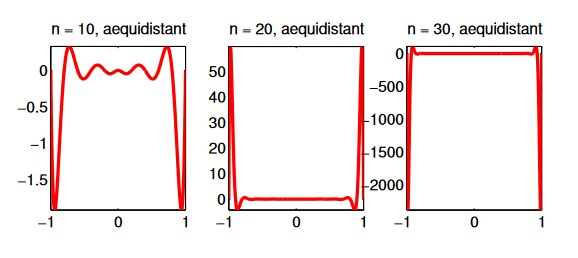
\includegraphics[scale=0.8]{rungespikes.jpg}
	\end{figure}
	Generell lässt sich keine generell optimale Knotenfolge finden. Allerdings kann $\Vert\omega_n\Vert$ minimiert werden. Dies geschieht durch die Chebychev-Punkte:
	\begin{definition}
		Die Chebychev-Polynome sind definiert als:
		$$T_n (X) := \cos(n\arccos x)$$
		Sie sind orthogonal bezüglich der Gewichtsfunktion $\frac{1}{\sqrt{1-x^2}}$. Sie besitzen die Nullstellen:
		$$x_i^{(n+1)}= \cos(\frac{2i+1}{2n+2}\pi)$$
		Diese werden auch als Chebychev-Punkte bezeichnet.
	\end{definition}
	\begin{theorem}[Dreiterm-Rekursion der Chebychev-Polynome]
		$T_0 = 1, T_1(x), T_n(x) = 2xT_{n-1}(x)-T_{n-2}(x)$
	\end{theorem}
	\begin{theorem}
		Für das Knotenpolynom $\omega_{n+1, cheb}$ zu den Chebychevpunkten gilt:
		$$\Vert\omega_{n+1,cheb} \Vert= 2^{-n}$$
	\end{theorem}
	Die theoretischen Überlegungen zur Bestimmung des Interpolationspolynom sind numerisch nicht stabil.
	\subsection{Auswertungsschemata}
	\begin{algorithm}[H]
		\caption{Auswertungschema von Aitken-Neville}
		\begin{algorithmic}
			\Require $n+1$ Stützstellen $(x_0, f_0), ..., (x_n, f_n)$, Auswertungsstelle $y$.
			\State Setze $P_i(y) \leftarrow f_i$ für $i=0, ..., n$
			\For{$i=1, ..., n$}
			\For{$j=0, ..., n-i$}
			\State $P_{j...j+i}(y) \leftarrow \frac{(y-x_j)P_{j+1...j+i}(y)-(y-x_{j+i})P_{j...j+i-1}(y)}{x_{j+i}- x_{j}}$
			\EndFor
			\EndFor
		\end{algorithmic}
	\end{algorithm}
	\begin{figure}[H]
		\centering
		\caption{Darstellung des Aitken-Neville-Schema}
		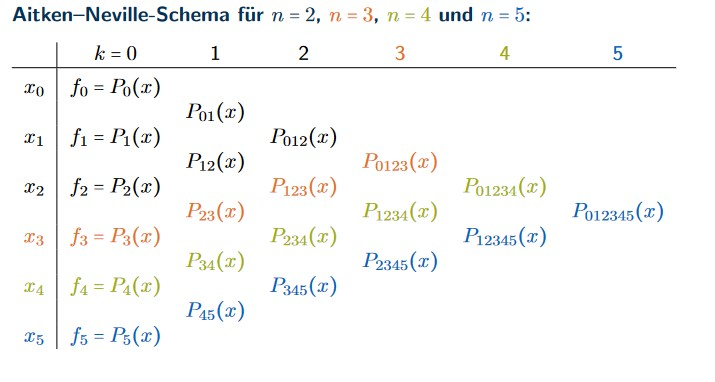
\includegraphics[scale=0.5]{aitken-neville.jpg}
	\end{figure}
	\begin{theorem}[Aufwand des Aitken-Neville-Verfahren]
		Für $l$ verschiedene Funktionen, $m$ Auswertungsstellen und $n+1$ Stützstellen beträgt der Aufwand für das Aitken-Neville-Schema $O(lmn^2)$.
	\end{theorem}
	Das Aitken-Neville Schema ist stabil aber langsam, wenn mehrere Stellen ausgwertet werden sollen. Um dies zu beschleunigen kann das 
	\begin{definition}[Newton-Darstellung eines Polynoms]
		Die Darstellung eines Polynoms in der Form:
		$$\pi_n(x) = c_0 + c_1(x-x_0) + c_2(x-x_0)(x-x_1) + ... + c_n(x-x_0)...(x-x_{n-1})$$
		Heißt \textbf{Newton'sche Darstellung}.
	\end{definition}
	\begin{algorithm}[H]
		\caption{Newton'sche Dividierte Differenzen}
		\begin{algorithmic}
			\Require $n+1$ Stützstellen $(x_0, f_0), ..., (x_n, f_n)$
			\State Setze $f[x_i]:=f_i$ für $i=0, ..., n$
			\For{$i=1, ..., n$}
			\For{$j=0, ..., n-i$}
			\State $f[x_j...x_{j+i}] \leftarrow \frac{f[x_{j+1}...x_{n-i}]-f[x_{j}...x_{n-i-1}]}{x_{j+i}- x_{j}}$
			\EndFor
			\EndFor
			\State $c_i \leftarrow f[x_0...f_i]$
		\end{algorithmic}
	\end{algorithm}
	\begin{algorithm}
		\caption{Horner-Schema}
		\begin{algorithmic}
			\Require Polynom in Newton-Darstellung mit Koeffizienten $c_0, ..., c_n$, Auswertungsstelle $y$.
			\State $p\leftarrow c_n$
			\For{$k=n-1, ..., 0$}
			\State $p \leftarrow p(y -x_k)+c_k$
			\EndFor
		\end{algorithmic}
	\end{algorithm}
	\begin{theorem}[Aufwand des Horner Schema]
		Für $l$ verschiedene Funktionen, $m$ Auswertungsstellen und $n+1$ Stützstellen beträgt der Aufwand für das Aitken-Neville-Schema $O(l(mn+n^2))$.
	\end{theorem}
	Allerdings ist das Horner-Schema \textbf{nicht stabil} für große $n$. Der Zugang über die baryzentrische Darstellung bietet dem Abhilfe und noch größere Effizienz.
	\begin{definition}[baryzentrische Gewichte]
		Wir definieren die \textbf{baryzentrischen Gewichte}  zu den Stützstellen $x_0, ..., x_n$ als:
		$$\lambda_i := \frac{1}{\prod_{k=0, k\neq i}^n(x_i-x_k)} = \frac{1}{\omega_{n+1}'(x_i)}$$
	\end{definition}
	\begin{theorem}[baryzentrische Darstellung des Lagrange-Polynoms]
		Für die Stützstellen $(x_0, f_0), ..., (x_n, f_n)$ hat das Interpolationspolynom die Form:
		$$\pi_n(x)=\omega_{n+1}(x)\sum_{i=1}^{n}\frac{\lambda_if_i}{x-x_i} = \frac{\sum_{i=1}^{n}\frac{\lambda_if_i}{x-x_i}}{\sum_{i=1}^{n}\frac{\lambda_i}{x-x_i}}$$
	\end{theorem}
	\begin{theorem}[Formen der baryzentrischen Gewichte] 
		Die Gewichte haben folgende Form (abhängig von der Wahl der Stützstellen):
		\begin{itemize}
			\item Äquidistant: ($x_i = -1 + ih, h=2/n$) 
			$$\lambda_i = \frac{(-1)^{n-i}}{h^n(n-i)!i!}$$
			\item Chebychev: ($x_i = \cos(\frac{2i+1}{2n+2}\pi)$)
			$$\lambda_i = (-1)^i\frac{2^n}{n+1}\sin(\frac{2i+1}{2n+2})$$
		\end{itemize}
	\end{theorem}
	\begin{theorem}
		Die Berechnung von $l$ Funktionen an $m$ Auswertungsstellen kostet $O(n^2+lmn)$ Schritte. Außerdem ist der Algorithmus stabil.
	\end{theorem}
	\subsection{Interpolationsfehler}
	\begin{definition}[Lebesque-Konstante]
		Wir definieren die \textbf{Lebesgue-Konstante} auf dem Intervall $[-1, 1]$ als:
		$$\Lambda_n := \Vert\sum_{i=0}^n|L_i(.)|\Vert_\infty$$
	\end{definition}
	\begin{theorem}
		Sei $\pi_n$ das Interpolationspolynom für $f$ und $\tilde{\pi_n}$ das für $\tilde{f}$ dann gilt:
		$$\Vert\pi_n-\tilde{\pi_n}\Vert \leq \Lambda_n\Vert f- \tilde{f}\Vert$$
	\end{theorem}
	\begin{definition}[Stetigkeitsmodul]
		Der \textbf{Stetigkeitsmodul} fon $f$ ist definiert als:
		$$\omega(f, \delta) := \sup_{|x-y|<\delta}|f(x)-f(y)|$$
	\end{definition}
	\begin{theorem}
		Für Lipschitz-stetige $f$ mit Lipschitzkonstante $L$ gilt: $\omega(f, \delta) \leq L\delta$.
	\end{theorem}
	\begin{theorem}[Interpolationsfehlerschranke durch Stetigkeitsmodul]
		Es gilt folgende Abschätzung für den Fehler der besten Approximation:
		$$\inf_{q\in \mathbb{P}^n}\Vert f-q\Vert \leq (1+\frac{\pi^2}{2})\omega(f, 1/n)$$
	\end{theorem}
	\begin{theorem}[Interpolationsfehlerschranke durch Bestappoximation]
		Sei $p^*$ die beste polynomielle Approximation an $f$, dann gilt folgende Fehlerabschätzung für das Interpolationspolynom $\pi_n$:
		$$\Vert f-\pi_n\vert \leq (1+\Lambda_n)\Vert f- p^*\Vert$$
	\end{theorem}	
	\begin{theorem}[Wachstumsschranken der Lebesgue-Konstanten]
		Die Lebesgue-Konstanten sind durch folgende Schranken begrenzt.
		\begin{itemize}
			\item Für Chebychev-Punkte gilt: 
			$$\frac{2}{\pi}\ln(n+1) \leq \Lambda_n \leq frac{2}{\pi}\ln(n+1)+1$$
			\item Für äquidistante Punkte gilt:
			$$Ce^{n/2}\leq \Lambda_n \sim \frac{2^{n+1}}{en\log n}$$
		\end{itemize}
	\end{theorem}
	\begin{theorem}[De la Vallée Poussin]
		Sei $f\in C$ und $p\in \mathbb{P}^n$ außerdem seien $x_0, ... x_{n+1}$ sodass: $(f(x_i)-p(x_i))(f(x_{i+1})- p(x_{i+1}) < 0)$. Dann gilt für die Bestapproximation $p^*$:
		$$\Vert p^*-f\Vert\geq \min |f(x_i)- p(x_i)|$$
	\end{theorem}
	\begin{theorem}[Oszillationstheorem]
		Sei $f\in C$ und $p\in \mathbb{P}^n$ zusätzlich seien $x_0, ...,x_{n+1}$, sodass:
		\begin{itemize}
			\item $f(x_i)-p(x_i) = - (f(x_{i+1})-p(x_{i+1}))$
			\item $|f(x_0)-p(x_0)| = \Vert f-p\Vert$
		\end{itemize}
		Dann ist $p$ die Bestapproximation von $f$ in $\mathbb{P}^n$. Man nennt $p$ auch \textbf{MinMax-Polynom}.
	\end{theorem}
	\subsection{Spline-Interpolation}
	\begin{definition}[Spline]
		Sei $\Delta = \{a=x_0 < x_1 < ... < x_n = b\}$ ein Gitter auf $[a, b]$ Dann sind die Splineräume von Grad $k$ definiert als:
		$$S_{\Delta, k} := \{v\in C^{k-1}([a, b]) : v|_{[x_i, x_{i+1}]}\in \mathbb{P}^k\}$$
		$$S_{\Delta, 0} : = \{v|_{[x_i, x_{i+1}]} \in \mathbb{P}^0\}$$
		Die Spline-Räume sind Vektorräume mit Dimension $n+k$.
	\end{definition}
	\begin{definition}[Unterarten des kubischen Splines]
		Um einen kubischen Spline $s\in S_{\Delta, 3}$ zu $f\in C^2$ zu berechnen benötigt man weitere Nebenbedingugnen:
		Dafür gibt es mehrere Möglichkeiten:
		\begin{itemize}
			\item Vollständiger Spline: $s'(x_0) = f'(x_0)$ und $s'(x_n) = f'(x_n)$
			\item Natürlicher Spline: $s''(x_0) = s''(x_n) = 0$
			\item Periodischer Spline: $s'(x_0) = s'(x_n)$ und $s''(x_0) = s''(x_n)$
		\end{itemize}
	\end{definition}
	\begin{definition}[Momentendarstellung eines kubischen Splines]
		Für $s \in S_{\Delta, 3}$ gilt $s'' \in S_{\Delta, 1}$. Seien die $N_i^2$ Basisfunktionen von $S_{\Delta, 1}$. Dann kann $s''$ dargestellt werden als:
		$$s''(x) = \sum_{i=0}^{n}m_iN_i^2(x)$$
		Die $m_i$ heißen \textbf{Momente}.
	\end{definition}
	\begin{definition}
		Aus den Momenten kann $s$ berechnet werden als:
		$$s(x)|_{[x_{i-1}, x_i]} = c_i ü d_i(x-\frac{x_{i-1}+x_i}{2}) +m_i\frac{(x-x_{i})^3}{6h_i} - m_{i-1}\frac{(x-x_{i-1})^3}{6h_i}$$
		Dabei sei $h_i = x_i -x_{i-1}$ und 
		$$c_i = \frac{f_i+f_{i-1}}{2}-\frac{h_i^2}{12}(m_i+m_{i-1})$$
		$$d_i = \frac{f_i-f_{i-1}}{h_i}-\frac{h_i}{6}(m_i-m_{i-1})$$
	\end{definition}
	Die Momente lassen sich folgendermaßen ausrechnen:
	\begin{theorem}
		Es gilt:
		$$\mu_i m_{i-1} + 2m_i + (1-\mu_i)m_{i+1} = b_i$$
		mit $\mu_i := h_i/(h_i+h_{i+1})$ und:
		$$b_i := \frac{6}{h_i+h_{i+1}}(\frac{f_{i+1}}{h_i} -f_i (1/h_i + 1/h_{i+1})+ f_{i-1}/h_i)$$
		Es gilt: 
		\begin{enumerate}
			\item Vollständiger kubischer Spline:
			$$\begin{bmatrix}
				2 & 1 & & & \\
				\mu_1 & 2 & 1-\mu_1 & & \\
				& \ddots& \ddots &\ddots &  \\
				& & \mu_{n-1} & 2 & 1-\mu_{n-1} \\
				& & & 1 & 2
			\end{bmatrix} \begin{pmatrix}
				m_0\\
				\vdots\\
				\vdots\\
				\vdots \\
				m_n
			\end{pmatrix} =  \begin{pmatrix}
				b_0\\
				\vdots\\
				\vdots\\
				\vdots \\
				b_n
			\end{pmatrix}$$
		\item Natürlicher kubischer Spline: Hier ist $m_0=m_n0$ und:
		$$\begin{bmatrix}
			2 & 1-\mu_1 & & & \\
			\mu_2 & 2 & 1-\mu_2 & & \\
			& \ddots& \ddots &\ddots &  \\
			& & \mu_{n-2} & 2 & 1-\mu_{n-2} \\
			& & & \mu_{n-1} & 2
		\end{bmatrix} \begin{pmatrix}
			m_1\\
			\vdots\\
			\vdots\\
			\vdots \\
			m_{n-1}
		\end{pmatrix} =  \begin{pmatrix}
			b_1\\
			\vdots\\
			\vdots\\
			\vdots \\
			b_{n-1}
		\end{pmatrix}$$
		\item periodischer Spline: Hier ist $m_n = m_0$
		$$\begin{bmatrix}
			2 & 1-\mu_n & & & \mu_n\\
			\mu_1 & 2 & 1-\mu_1 & & \\
			& \ddots& \ddots &\ddots &  \\
			& & \mu_{n-2} & 2 & 1-\mu_{n-2} \\
			&1-\mu_{n-1} & & \mu_{n-1} & 2
		\end{bmatrix} \begin{pmatrix}
			m_0\\
			\vdots\\
			\vdots\\
			\vdots \\
			m_{n-1}
		\end{pmatrix} =  \begin{pmatrix}
			b_0\\
			\vdots\\
			\vdots\\
			\vdots \\
			b_{n-1}
		\end{pmatrix}$$
		\end{enumerate}
	\end{theorem}
	\begin{theorem}[Fehler der Spline-Interpolation]
		Für $f\in C^4$ und den vollständigen kubischen Spline $s\in S_{\Delta, 3}$gilt: $$ \Vert (f-s)^{(k)}\Vert \leq Ch^{4-k} \Vert f^{(4)}\Vert $$
		Dabei ist $h := \max |x_{i+1} -x_i|$.
	\end{theorem}
	\begin{definition}[Kardinal-Spline-Basisfunktionen]
		$S_{\Delta, 3}$ kann durch folgende Basis dargestellt werden:
		\begin{itemize}
			\item $K'_{-1} (x_0)=1, K_{-1}(x_i) = 0, K'_{-1}(x_n) = 0$
			\item $K_i(x_j) = \delta_{ij}, K'_{i}(x_0) = K'_{i}(x_n)= 0$
			\item \item $K'_{n+1} (x_0)=1, K_{-1}(x_i) = 0, K'_{-1}(x_n) = 0$
		\end{itemize}
	\end{definition}
	Da diese globale Träger haben wird alternativ eine andere Basisdarstellung gewählt:
	\begin{definition}[B-Splines]
		Die \textbf{B-Spline Basisfunktionen} von $S_{\Delta, l}$ sind definiert durch die $B_{i, l+1}, i=1-l, n$:
		$$B_i, 1(x) := \begin{cases}
			1 & \text{falls }x \in [x_{i-1}, x_{i}],\\
			0 & \text{sonst} 
		\end{cases}$$
		$$B_{i, k} := \frac{x-x_{i-1}}{x_{i+k-2}-x_{i-1}}B_{i, k-1}+  \frac{x_{i+k-1}-x}{x_{i+k-1}-x_{i}}B_{i+1, k-1}$$
	\end{definition}
	\begin{theorem}[Nützliche EIgenschaften der B-Spline Basisifunktionen]
		Die B-Spline Basisfunktionen erfüllen folgende Eigenschaften:
		\begin{enumerate}
			\item $\text{supp} B_{i, k} \subset [s_{i-1}, x_{i+k-1}]$
			\item $B_{i, k} \geq 0$
			\item $\sum_{i=2-k}^n B_{i, k} = 1$
		\end{enumerate}
	\end{theorem}
	\section{Quadratur}
	\begin{definition}[Quadraturformel]
		Eine \textbf{Quadraturformel} hat im allgemeinen die Form:
		$$Q^a_b(f) := \sum_{i=0}^{n}w_if(x_i)$$
		Sind die Gewichte $w_i := \int_a^bL_i(x)dx$, so ist die Quadraturformel vom \textbf{Interpolationstyp}.
	\end{definition}
	\begin{definition}[Exaktheitsgrad]
		Eine Quadraturformel hat den \textbf{Exaktheitsgrad} $n$ falls sie für alle Polynome in $\mathbb{P}^n$ exakt ist, aber nicht für $x^{n+1}$
	\end{definition}
	\begin{definition}[symmetrische Quadraturformel]
		Eine \textbf{symmetrische QF} erfüllt:
		$$w_i = w_{n-i}, x_i-a=b-x_{n-i}$$
	\end{definition}
	\begin{theorem}[Aussagen über den Exaktheitsgrad]
		\begin{enumerate}
			\item Jede QF vom Interpolationstyp und mit $n+1$ Knoten hat mind. Exaktheitsgrad $n$. 
			\item Außerdem ist der Exaktheitsgrad einer symmetrischen Quadraturformel ungerade.
			\item Jede QF mit $n+1$ Knoten und mindestens Exaktheitsgrad $n$ muss vom Interpolationstyp sein.
			\item Falls die Gewichte einer QF durch Interpolation bestimmt sind und die Knoten symmetrisch angeordnet sind. Dann ist die QF auch symmetrisch
			\item Eine QF mit $n+1$ Knoten hat maximal den Exaktheitsgrad $2n+1$.
			\item Die QF mit Exaktheitsgrad $2n+1$ bei $n+1$ Knoten ist eindeutig.
			\item Für eine QF mit Exaktheitsgrad $\geq 2n$ müssen alle Gewichte positiv sein.
		\end{enumerate}
	\end{theorem}
	\subsection{Newton-Cotes-Formel}
	\begin{definition}[Newton-Cotes QF]
		Bei der Newton Cotes QF sind die Punkte äquidistant verteilt, man unterscheidet zwischen:
		\begin{enumerate}
			\item Der geschlossenen Newton Cotes Formel:
			 $$x_i = a+ ih, h= \frac{b-a}{n}$$
			\item Der offenen Newton Cotes Formel:
			$$x_i = a+ (i+1)h, h= \frac{b-a}{n+2}$$
		\end{enumerate}
	\end{definition}
	Geschlossene Quadraturformeln:
	\begin{center}
		\begin{tabular}{ c c c c}
			\textbf{Name} &   \textbf{Gewichte} & \textbf{Fehler} & \textbf{Exaktheitsgrad}\\
			Trapez  & $w_1=w_2=\frac{1}{2}$ & $-\frac{h^3}{12}f''(\xi)$ & 1\\
			Cavalieri-Simpson & $w_0=\frac{1}{6}(b-a), w_1 = \frac{4}{6}(b-a)$ & $-\frac{h^5}{90}f^{(4)}(\xi)$& 3\\
			Simpson 3/8 & $w_0 = \frac{3}{8}\frac{b-a}{3}, w_1 = \frac{9}{8}\frac{b-a}{3}$ & $-\frac{3h^5}{80}f^{(4)}(\xi)$ & 3 \\
			Milne & $w_1=\frac{7}{90}, w_2=\frac{32}{90}, w_3=\frac{12}{90}$ & $-\frac{8}{945}h^7f^{(6)}(\xi)$ &5
		\end{tabular}
	\end{center}
	\begin{theorem}[Fehler allgemeiner Newton-Cotes-Formeln]
		Sei $n$ gerade und $f\in C^{n+2}$, dann gilt für den Quadraturfehler:
		$$E_n(f) = \frac{M_n}{(n+2)!}h^{n+3}f^{(n+2)}(\xi)$$
		Dabei ist:
		$$M_n = \begin{cases}
			\int_0^nt\hat{\omega}_{n+1}(t)dt & \text{für gechlossene QF}\\
			\int_{-1}^{n+1}t\hat{\omega}_{n+1}(t)dt & \text{für offene QF}\\
		\end{cases}$$
		Wobei $\hat{\omega}_{n+1}(t) := \prod_{i=0}^n(t-i)$.
		Für $n$ ungerade gilt:
		$$E_n(f) = \frac{K_n}{(n+1)!}h^{n+2}f^{(n+1)}(\xi)$$
		Dabei ist:
		$$K_n = \begin{cases}
			\int_0^n\hat{\omega}_{n+1}(t)dt & \text{für gechlossene QF}\\
			\int_{-1}^{n+1}\hat{\omega}_{n+1}(t)dt & \text{für offene QF}\\
		\end{cases}$$
	\end{theorem}
	Die Newton-Cotes Formeln können auf Teilintervalle angewandt werden.
	\begin{theorem}
		Für zusammengestzte Newton-Cotes Formeln mit $m$ Teilintervallen verliert die Fehlerabschätzung eine $h$-Potenz es gilt mit $H=\frac{b-a}{m}$. \\
		Für $n$ gerade:
		$$E_n(f) = \frac{(b-a)M_n}{\gamma^{n+3}_n(n+2)!}H^{n+2}f^{(n+2)}(\xi)$$
		Für $n$ ungerade:
		$$E_n(f) = \frac{(b-a)K_n}{\gamma^{n+2}_n(n+1)!}H^{n+1}f^{(n+1)}(\xi)$$
		Wobei $\gamma_n= \begin{cases}
			n+2 & \text{für QF offen} \\
			n & \text{für QF geschlossen}
		\end{cases}$.
	\end{theorem}
	\subsection{Gauß-Quadratur}
	\begin{theorem}[Dreiterm-Rekursion]
		Die orthogonalen Polynome für ein Skalarprodukt $\langle., .\rangle$ werden bestimmt durch:
		$$p_{k+1} = (x-\alpha_k)p_k(x) - \beta_kp_{k-1}(x)$$
		$$p_{-1}=0, p_0(x)=1$$
		und:
		$$\alpha_k=\frac{\langle x p_k, p_k\rangle}{\langle p_k, p_k\rangle}, \beta_k=\frac{\langle p_k, p_k\rangle}{\langle p_{k-1}, p_{k-1}\rangle}$$
	\end{theorem}
	\begin{definition}[Legendre Polynome]
		Die Legendre Polynome sind orthogonal zu dem Skalarprodukt mit Gewichtugnsfunktion $w=1$. 
		$$L_0(x)=1, L_1(x)=x$$
		$$L_{k+1}(x) = \frac{2k+1}{k+1}xL_k(x) -\frac{k}{k+1}L_{k+1}(x)$$
		Sie lassen sich auch folgendermaßen darstellen:
		$$L_k(x) = \frac{(-1)^k}{2^k k!} \frac{d^k}{dx^k}(1-x^2)^k$$
	\end{definition}
	\begin{definition}[Gegenbauer-Polynome]
		Die Gegenbauer-Polynome $G^\alpha_k$ sind die Orthogonalpolynome für $w(x) = (1-x^2)^{\alpha-1/2}$. \\
		Die Legendre und Chebchev-Polynome sind Spezialfälle für $\alpha=1/2$ und $\alpha=0$. Außerdem gilt:
		$$L'_n = G^{3/2}_{n-1}(x)$$
	\end{definition}
	\begin{theorem}
		Die Dreiterm-Rekursion für die $G^{3/2}_k$ lautet:
		$$G^{3/2}_0(x)=1, G^{3/2}_1(x)=3x$$
		$$G^{3/2}_{k+1}(x) = \frac{2k+3}{k+1}xG^{3/2}_k(x) -\frac{k+2}{k+1}G^{3/2}_{k+1}(x)$$
	\end{theorem}
	\begin{definition}[Laguerre-Polynome]
		Laguerre-Polynome $L_k$ sind orthogonal zu $w(x) = e^{-x}$.
	\end{definition}
	\begin{theorem}
		Die Dreiterm-Rekursion für die Laguerre Polynome lautet:
		$$L_{-1}(x)=0, L_1(x)= 1$$
		$$L_{k+1}(x) = (2k+1-x)L_k(x) - k^2L_{k-1}(x)$$
		Sie lassen sich auch folgendermaßen darstellen:
		$$L_k(x)= e^x\frac{d^k}{dx^k}(e^{-x}x^k)$$
	\end{theorem}
	\begin{definition}[Hermite-Polynome]
		Die Hermite-Polynome sind orthogonal zur Gewichtsfunktion $w(x) = e^{-x^2}$.
	\end{definition}
	\begin{theorem}
		Die Hermite-Polynome folgen der Dreiterm-Rekursion:
		$$H_{-1}(0), H_0(x)=1$$
		$$H_{k+1}(x)=2xH_k(x)-2kH_{k-1}(x)$$
	\end{theorem}
	\begin{theorem}[Quadratur-Satz von Jacobi]
		Eine QF mit $n+1$ Knoten ist had Exaktheitsgrad $n+m$, genau dann wenn das Knotenpolynom $\omega_{n+1}$ orthogonal auf $\mathbb{P}^{m-1}$ steht.
	\end{theorem}
	\begin{definition}[Gauß-(Lobatto)-Quadratur]
		Bei der Gaußquadratur sind die Stützstellen die Nullstellen von $L_{n+1}$ und die Gewichte:
		$$w_i = \frac{2}{(1-x_i^2)(L'_{n+1}(x_i))^2}$$
		Für die Gauß-Lobatto Quadratur setzt man $x_0=-1, x_n=1$ an die Endpunkte des Intervalls. Die anderen Punkte sind die Nullstellen des $G_{n-1}^{3/2}= L'_n(x)$-Polynoms.
		Die Gewichte sind:
		$$w_i=\frac{2}{n(n+1)}\frac{1}{[L_n(x)]^2}$$
	\end{definition}
	\begin{definition}[Laguerre-Quadratur]
		Um auf dem Intervall $(0, \infty)$ zu integrieren benutzt man die Laguerre-Quadratur. Dazu definiert man $\phi(x) = e^x f(x)$ und es gilt $\int_0^\infty e^{-x}\phi(x) = I(f)$
		Man quadriere nun $\phi$ mit den Stützstellen als den Nullstellen des Laguerre-Polynoms: $L_{n+1}$ und den Gewichten:
		 $$w_i = \frac{x_i}{(n+2)^2[L_{n+2}(x_i)]^2}$$
	\end{definition}
	\begin{definition}[Hermite-Quadratur]
		Um auf dem Intervall $(-\infty, \infty)$ zu integrieren benutzt man die Laguerre-Quadratur. Dazu definiert man $\phi(x) = e^{-x^2} f(x)$ und es gilt $\int_0^\infty e^{-x^2}\phi(x) = I(f)$
		Man quadriere nun $\phi$ mit den Stützstellen als den Nullstellen des Hermite-Polynoms: $H_{n+1}$ und den Gewichten:
		 $$w_i = \frac{2^{n+2}(n+1)!\sqrt(\pi)}{[H_{n+2}(x_i)]^2}$$
	\end{definition}
	\subsection{Extrapolation}
	\begin{definition}[Richardson-Extrapolation]
		Ein numerisches Schema $A$ mit einer Entwicklung 
		$$A(h) = q_0 +q_1h + ... + q_kh^k+ O(h^{k+1})$$
		lässt sich durch extrapolation verbessern. Das Extrapolationsschema ist:
		$$A_{k, 0} = A(\delta^kh)$$
		$$A_{k, l+1} = \frac{A_{k, l} - \delta^{l+1}A_{k-1, l}}{1-\delta^{l+1}}$$
	\end{definition}
	\begin{theorem}
		Durch das Anwenden des Extrapolationsschemas mit $\delta \in (0,1)$ erhält man:
		$$A_{k, l}(h) = q_0 + O((\delta^kh)^{l+1})$$
	\end{theorem}
	\begin{theorem}[Euler-MacLaurin-Formel]
		Sei $f\in C^{2n+2}$ und $q_0 = I(f)$ dann gilt für die zusammengestzte Trapezregel:
		$$I_{1,m}(f) = q_0 + \sum_{i=1}^{n}\alpha_{2i}h^{2i}_m + O(h_m^{2n+2})$$
	\end{theorem}
	\begin{algorithm}
		\caption{Romberg-Quadratur}
		\begin{algorithmic}
			\Require $f$
			\For{$k=1, ..., n$}
			\State $A_{k, 0} \leftarrow I_{1, 2^k}(f)$
			\EndFor
			\For{$l=1, ..., n$}
			\For{$k=l, ..., n$}
				\State $A_{k, l} \leftarrow \frac{4^{l+1}A_{k, l-1} -A_{k-1, l-1}}{4^{l+1}-1}$
			\EndFor
			\EndFor
		\end{algorithmic}
	\end{algorithm}
	\section{Lösung nichtlinearer Gleichungssysteme}
	\begin{algorithm}
		\caption{Bisektionsverfahren}
		\begin{algorithmic}
			\Require $f, x_0, x_1$ und $f(x_0)f(x_1) < 0$
			\For{$k=1, 2, ...$}
			\State $x_{k+1} \leftarrow \frac{1}{2}(x_k + x_{k-1})$
			\If{$f(x_{k+1})f(x_{k-1}) < 0$}
			\State $x_k \leftarrow x_{k-1}$
			\EndIf
			\EndFor 
		\end{algorithmic}
	\end{algorithm}
	\begin{theorem}[Konvergenz des Bisektionsverfahren]
		Das Bisektionsverfahren konvergiert gegen eine Nullstelle $x^*$:
		$$|x^* - x_{k+1}| \leq 2^{-k}|x_0-x_1|$$
	\end{theorem}
	\begin{algorithm}
		\caption{Sekantenverfahren}
		\begin{algorithmic}
			\Require $f, x_0, x_1$
			\For{$k=1, 2, ...$}
			\State $x_{k+1} = x_k - \frac{x_k-x_{k-1}}{f(x_k)- f(x_{k-1})}f(x_k)$
			\EndFor 
		\end{algorithmic}
	\end{algorithm}
	Das Sekantenverfahren konvergiert, falls die Startwerte bereits nahe an einer Nullstelle $x^*$ liegen recht schnell, allerdings können Fehler auftreten, falls $f(x_{k-1}) = f(x_k)$.
	\begin{algorithm}
		\caption{Regula Falsi}
		\begin{algorithmic}
			\Require $f, x_0, x_1$ und $f(x_0)f(x_1) < 0$
			\For{$k=1, 2, ...$}
			\State $x_{k+1} = x_k - \frac{x_k-x_{k-1}}{f(x_k)- f(x_{k-1})}f(x_k)$
			\If{$f(x_{k+1})f(x_{k-1}) < 0$}
			\State $x_k \leftarrow x_{k-1}$
			\EndIf
			\EndFor
		\end{algorithmic}
	\end{algorithm}
	\begin{theorem}
		Das Regula Falsi Verfahren konvergiert immer.
	\end{theorem}
	\begin{definition}[Konvergenzordnung]
		Eine Folge $(x_k)_{k\in \mathbb{N}}$ heißt konvergent von Ordnung $p\geq 1$ gegen $x^*$ falls $c < \infty$ exisitiert, sodass:
		$$\Vert x_{k+1} - x^*\Vert \leq c\Vert x_k -x^*\Vert^p$$
		Für $p=1$ muss zusätzlich $c<1$ gelten.
	\end{definition}
	\begin{theorem}[Konvergenz einer Fixpunktiteration]
		Sei $\Phi\in C^1$ und $x^*$ ein Fixpunkt. Die Fixpunktiteration von $\Phi$ in der Umgebung von $x^*$ ist:
		\begin{itemize}
			\item konvergent falls $|\Phi'(x^*)| < 1$
			\item divergent falls $|\Phi'(x^*)| > 1$
			\item konvergent von ordnung $p \geq 2$ falls $\Phi \in C^p$ und:
			$$\Phi^{(l)}(x^*) = 0, \ \ \ l=1, 2, ..., p-1$$
		\end{itemize}
	\end{theorem}
	\begin{algorithm}
		\caption{Newton-Verfahren}
		\begin{algorithmic}
			\Require $F\in C^1$, Startwert $x_0$.
			\For{$k=0, 1, ...$}
			\State Löse $DF(x_k)\Delta x_k = F(x_k)$
			\State $x_{k+1} \leftarrow x_k - \Delta x_k$
			\EndFor
		\end{algorithmic}
	\end{algorithm}
	\begin{theorem}
		Falls für $DF$ ein $\omega$ existiert, sodass:
		$$\Vert DF(x)^{-1}(DF(x+sv)- DF(x))v\Vert \leq s\omega\Vert v\Vert^2$$
		Dann gilt für alle Startwerte $x_0 \in B_{\frac{2}{\omega}(x^*)}$, dass das Newton-Verfahren mindestens quadratisch gegen $x^*$ konvergiert.
	\end{theorem}
	\begin{algorithm}[H]
		\caption{gedämpftes Newton-Verfahren}
		\begin{algorithmic}
		
			\Require $F\in C^1$, Startwert $x_0$, Dämpfungsparameter $\gamma$.
			\For{$k=0, 1, ...$}
			\State Löse $DF(x_k)\Delta x_k = F(x_k)$
			\State $x_{k+1} \leftarrow x_k - \gamma\Delta x_k$
			\EndFor
		\end{algorithmic}
	\end{algorithm}
	Der Dämpfungsparameter kann natürlich in jedem Schritt angepasst werden.
	\begin{theorem}
		Das gedämpfte Newtonverfahren für $\Phi$ mit Parameter $\gamma$ ist äquivalent zum Newtonverfahren für $\Phi_\gamma(x) = (1-\gamma)x + \gamma \Phi(x)$ 
	\end{theorem}
	\begin{definition}[Inexaktes Newtonverfahren]
		Hier wird $DF(x_k)\Delta x_k = F(x_k)$ in jedem Schritt nur näherungsweise gelöst.
	\end{definition}
	\begin{definition}[Newton-artiges Verfahren]
		Hier wird $DF(x_k)$ durch $M_k$ approximiert.
	\end{definition}
	\begin{theorem}[Dennis-Moré-Bedingugn]
		Für ein Newton-artiges Verfahren ist folgendes equivalent:
		\begin{itemize}
			\item Die Konvergenz ist superlinear und $F(x^*) = 0$
			\item $\Vert (M_k - DF(x_k)\Delta x_k )\Vert = o(\Vert \Delta x_k \Vert)$
		\end{itemize}
	\end{theorem}
	\begin{theorem}[Sherman-Morrison-Formel]
		Sei $A$ invertierber, dann ist $A+uv^T$ genau dann invertierbar, wenn $1 + v^TAu \neq 0$. Dann gilt:
		$$(A+uv^T)^{-1} = A^{-1} - \frac{A^{-1}uv^TA^{-1}}{1+v^TA^{-1}u}$$
	\end{theorem}
	\begin{algorithm}
		\caption{BFGS-Algorithmus}
		\begin{algorithmic}
			\Require Startwert $x_0$ und Startinverse $B_0^{-1}$ (Approximation von $DF^{-1}(x_0)$, oder häufig auch identität), Schrittweiten $\lambda_k$
			\For{$k=0,1, 2, ...$}
			\State $\Delta x \leftarrow -\lambda_kB_k^{-1}F(x_k)$
			\State $x_{k+1}\leftarrow x_k + \Delta x$
			\State $\Delta F \leftarrow F(x_{k+1}) -F(x_k)$
			\State $B_{k+1}^{-1} \leftarrow B_{k+1}^{-1} + (\Delta x -B^{-1}_k\Delta F)\frac{\Delta x^T B^{-1}_{k}}{\Delta x^T B^{-1}_{k}\Delta F}$
			\EndFor 
		\end{algorithmic}
	\end{algorithm}
\end{document}